\documentclass[1p]{elsarticle_modified}
%\bibliographystyle{elsarticle-num}

%\usepackage[colorlinks]{hyperref}
%\usepackage{abbrmath_seonhwa} %\Abb, \Ascr, \Acal ,\Abf, \Afrak
\usepackage{amsfonts}
\usepackage{amssymb}
\usepackage{amsmath}
\usepackage{amsthm}
\usepackage{scalefnt}
\usepackage{amsbsy}
\usepackage{kotex}
\usepackage{caption}
\usepackage{subfig}
\usepackage{color}
\usepackage{graphicx}
\usepackage{xcolor} %% white, black, red, green, blue, cyan, magenta, yellow
\usepackage{float}
\usepackage{setspace}
\usepackage{hyperref}

\usepackage{tikz}
\usetikzlibrary{arrows}

\usepackage{multirow}
\usepackage{array} % fixed length table
\usepackage{hhline}

%%%%%%%%%%%%%%%%%%%%%
\makeatletter
\renewcommand*\env@matrix[1][\arraystretch]{%
	\edef\arraystretch{#1}%
	\hskip -\arraycolsep
	\let\@ifnextchar\new@ifnextchar
	\array{*\c@MaxMatrixCols c}}
\makeatother %https://tex.stackexchange.com/questions/14071/how-can-i-increase-the-line-spacing-in-a-matrix
%%%%%%%%%%%%%%%

\usepackage[normalem]{ulem}

\newcommand{\msout}[1]{\ifmmode\text{\sout{\ensuremath{#1}}}\else\sout{#1}\fi}
%SOURCE: \msout is \stkout macro in https://tex.stackexchange.com/questions/20609/strikeout-in-math-mode

\newcommand{\cancel}[1]{
	\ifmmode
	{\color{red}\msout{#1}}
	\else
	{\color{red}\sout{#1}}
	\fi
}

\newcommand{\add}[1]{
	{\color{blue}\uwave{#1}}
}

\newcommand{\replace}[2]{
	\ifmmode
	{\color{red}\msout{#1}}{\color{blue}\uwave{#2}}
	\else
	{\color{red}\sout{#1}}{\color{blue}\uwave{#2}}
	\fi
}

\newcommand{\Sol}{\mathcal{S}} %segment
\newcommand{\D}{D} %diagram
\newcommand{\A}{\mathcal{A}} %arc


%%%%%%%%%%%%%%%%%%%%%%%%%%%%%5 test

\def\sl{\operatorname{\textup{SL}}(2,\Cbb)}
\def\psl{\operatorname{\textup{PSL}}(2,\Cbb)}
\def\quan{\mkern 1mu \triangleright \mkern 1mu}

\theoremstyle{definition}
\newtheorem{thm}{Theorem}[section]
\newtheorem{prop}[thm]{Proposition}
\newtheorem{lem}[thm]{Lemma}
\newtheorem{ques}[thm]{Question}
\newtheorem{cor}[thm]{Corollary}
\newtheorem{defn}[thm]{Definition}
\newtheorem{exam}[thm]{Example}
\newtheorem{rmk}[thm]{Remark}
\newtheorem{alg}[thm]{Algorithm}

\newcommand{\I}{\sqrt{-1}}
\begin{document}

%\begin{frontmatter}
%
%\title{Boundary parabolic representations of knots up to 8 crossings}
%
%%% Group authors per affiliation:
%\author{Yunhi Cho} 
%\address{Department of Mathematics, University of Seoul, Seoul, Korea}
%\ead{yhcho@uos.ac.kr}
%
%
%\author{Seonhwa Kim} %\fnref{s_kim}}
%\address{Center for Geometry and Physics, Institute for Basic Science, Pohang, 37673, Korea}
%\ead{ryeona17@ibs.re.kr}
%
%\author{Hyuk Kim}
%\address{Department of Mathematical Sciences, Seoul National University, Seoul 08826, Korea}
%\ead{hyukkim@snu.ac.kr}
%
%\author{Seokbeom Yoon}
%\address{Department of Mathematical Sciences, Seoul National University, Seoul, 08826,  Korea}
%\ead{sbyoon15@snu.ac.kr}
%
%\begin{abstract}
%We find all boundary parabolic representation of knots up to 8 crossings.
%
%\end{abstract}
%\begin{keyword}
%    \MSC[2010] 57M25 
%\end{keyword}
%
%\end{frontmatter}

%\linenumbers
%\tableofcontents
%
\newcommand\colored[1]{\textcolor{white}{\rule[-0.35ex]{0.8em}{1.4ex}}\kern-0.8em\color{red} #1}%
%\newcommand\colored[1]{\textcolor{white}{ #1}\kern-2.17ex	\textcolor{white}{ #1}\kern-1.81ex	\textcolor{white}{ #1}\kern-2.15ex\color{red}#1	}

{\Large $\underline{10_{67}~(K10a_{37})}$}

\setlength{\tabcolsep}{10pt}
\renewcommand{\arraystretch}{1.6}
\vspace{1cm}\begin{tabular}{m{100pt}>{\centering\arraybackslash}m{274pt}}
\multirow{5}{120pt}{
	\centering
	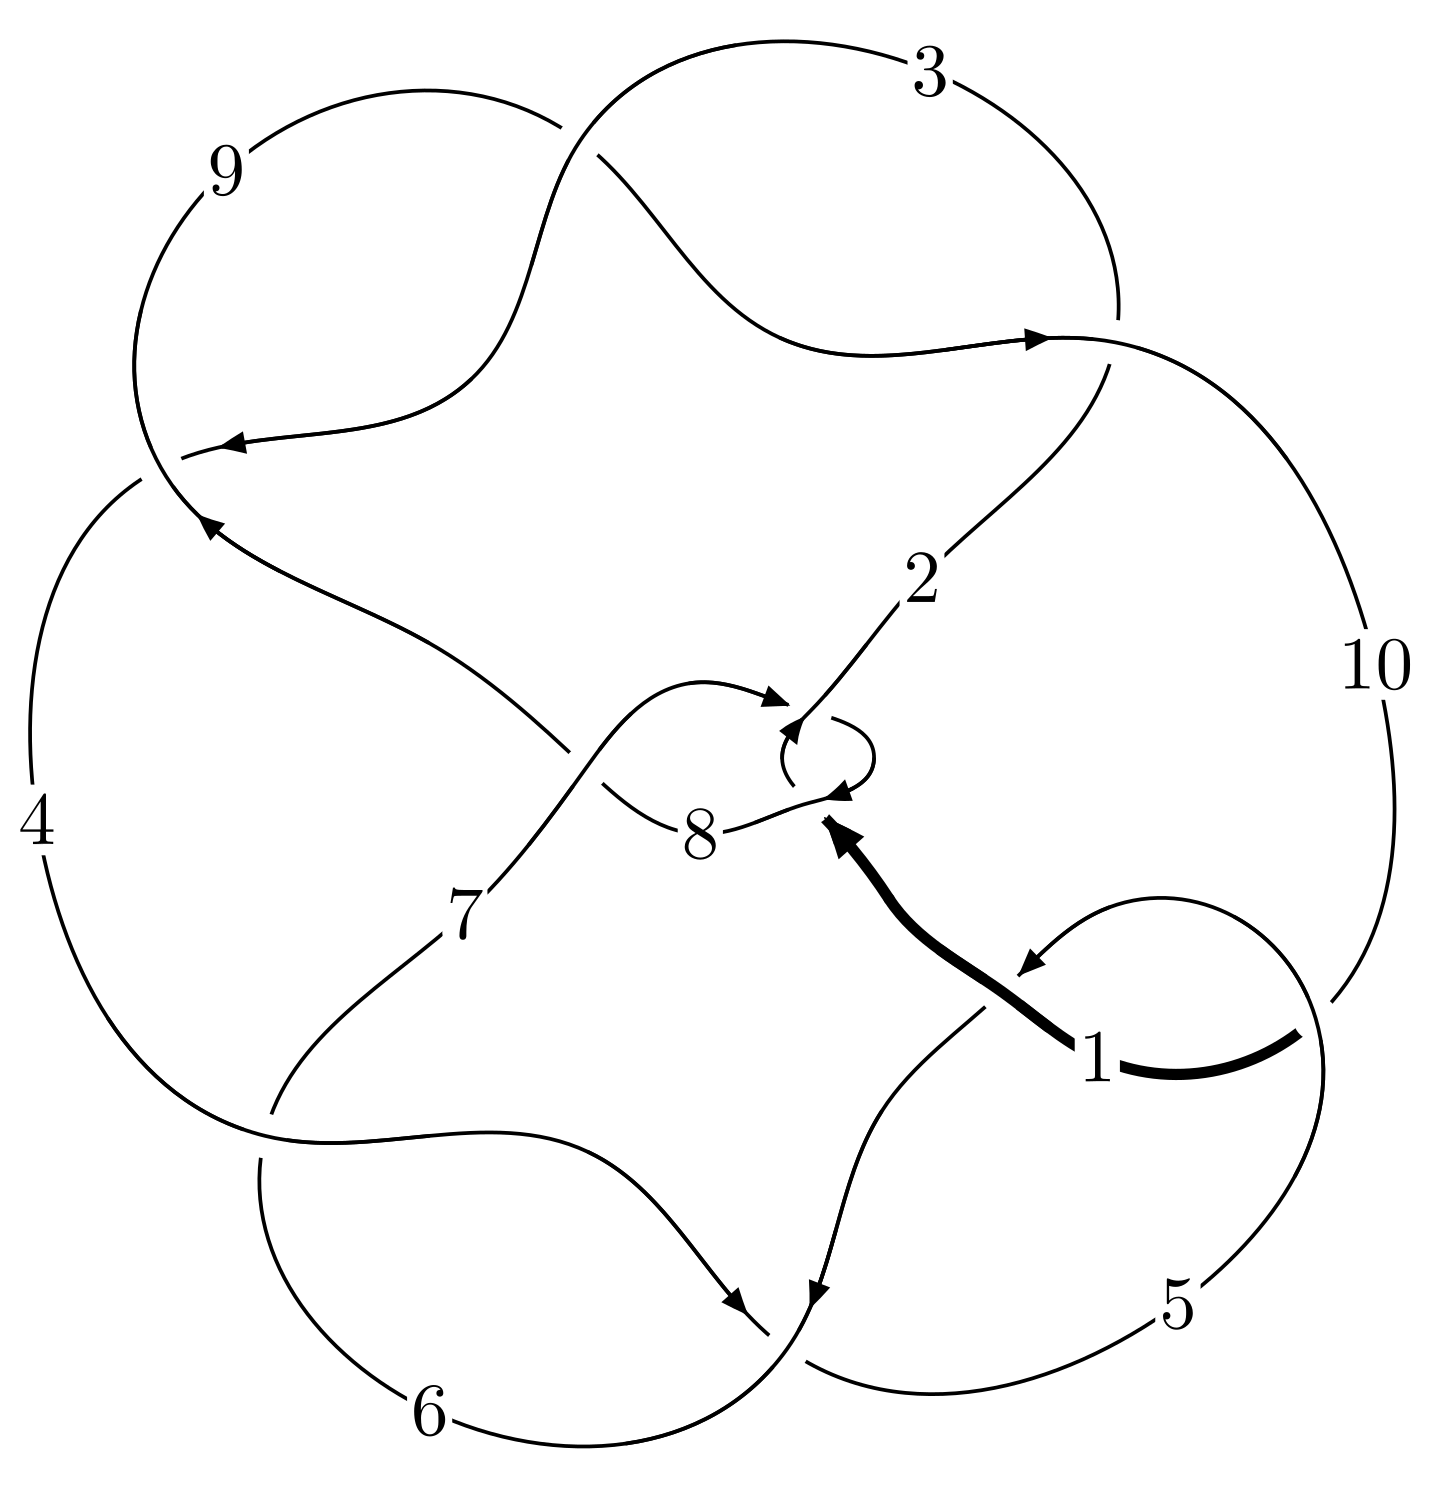
\includegraphics[width=112pt]{../../../GIT/diagram.site/Diagrams/png/151_10_67.png}\\
\ \ \ A knot diagram\footnotemark}&
\allowdisplaybreaks
\textbf{Linearized knot diagam} \\
\cline{2-2}
 &
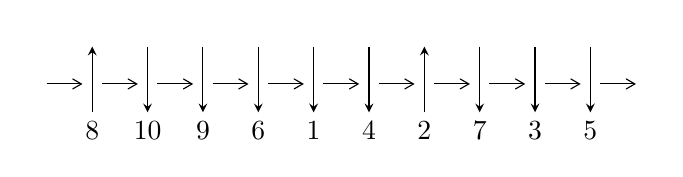
\begin{tikzpicture}[x=20pt, y=17pt]
	% nodes
	\node (C0) at (0, 0) {};
	\node (C1) at (1, 0) {};
	\node (C1U) at (1, +1) {};
	\node (C1D) at (1, -1) {8};

	\node (C2) at (2, 0) {};
	\node (C2U) at (2, +1) {};
	\node (C2D) at (2, -1) {10};

	\node (C3) at (3, 0) {};
	\node (C3U) at (3, +1) {};
	\node (C3D) at (3, -1) {9};

	\node (C4) at (4, 0) {};
	\node (C4U) at (4, +1) {};
	\node (C4D) at (4, -1) {6};

	\node (C5) at (5, 0) {};
	\node (C5U) at (5, +1) {};
	\node (C5D) at (5, -1) {1};

	\node (C6) at (6, 0) {};
	\node (C6U) at (6, +1) {};
	\node (C6D) at (6, -1) {4};

	\node (C7) at (7, 0) {};
	\node (C7U) at (7, +1) {};
	\node (C7D) at (7, -1) {2};

	\node (C8) at (8, 0) {};
	\node (C8U) at (8, +1) {};
	\node (C8D) at (8, -1) {7};

	\node (C9) at (9, 0) {};
	\node (C9U) at (9, +1) {};
	\node (C9D) at (9, -1) {3};

	\node (C10) at (10, 0) {};
	\node (C10U) at (10, +1) {};
	\node (C10D) at (10, -1) {5};
	\node (C11) at (11, 0) {};

	% arrows
	\draw[->,>={angle 60}]
	(C0) edge (C1) (C1) edge (C2) (C2) edge (C3) (C3) edge (C4) (C4) edge (C5) (C5) edge (C6) (C6) edge (C7) (C7) edge (C8) (C8) edge (C9) (C9) edge (C10) (C10) edge (C11) ;	\draw[->,>=stealth]
	(C1D) edge (C1U) (C2U) edge (C2D) (C3U) edge (C3D) (C4U) edge (C4D) (C5U) edge (C5D) (C6U) edge (C6D) (C7D) edge (C7U) (C8U) edge (C8D) (C9U) edge (C9D) (C10U) edge (C10D) ;
	\end{tikzpicture} \\
\hhline{~~} \\& 
\textbf{Solving Sequence} \\ \cline{2-2} 
 &
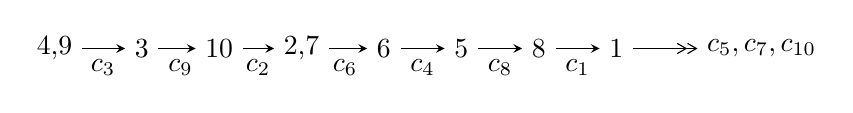
\begin{tikzpicture}[x=28pt, y=7pt]
	% node
	\node (A0) at (-1/8, 0) {4,9};
	\node (A1) at (1, 0) {3};
	\node (A2) at (2, 0) {10};
	\node (A3) at (49/16, 0) {2,7};
	\node (A4) at (33/8, 0) {6};
	\node (A5) at (41/8, 0) {5};
	\node (A6) at (49/8, 0) {8};
	\node (A7) at (57/8, 0) {1};
	\node (C1) at (1/2, -1) {$c_{3}$};
	\node (C2) at (3/2, -1) {$c_{9}$};
	\node (C3) at (5/2, -1) {$c_{2}$};
	\node (C4) at (29/8, -1) {$c_{6}$};
	\node (C5) at (37/8, -1) {$c_{4}$};
	\node (C6) at (45/8, -1) {$c_{8}$};
	\node (C7) at (53/8, -1) {$c_{1}$};
	\node (A8) at (9, 0) {$c_{5},c_{7},c_{10}$};

	% edge
	\draw[->,>=stealth]	
	(A0) edge (A1) (A1) edge (A2) (A2) edge (A3) (A3) edge (A4) (A4) edge (A5) (A5) edge (A6) (A6) edge (A7) ;
	\draw[->>,>={angle 60}]	
	(A7) edge (A8);
\end{tikzpicture} \\ 

\end{tabular} \\

\footnotetext{
The image of knot diagram is generated by the software ``\textbf{Draw programme}" developed by Andrew Bartholomew(\url{http://www.layer8.co.uk/maths/draw/index.htm\#Running-draw}), where we modified some parts for our purpose(\url{https://github.com/CATsTAILs/LinksPainter}).
}\phantom \\ \newline 
\centering \textbf{Ideals for irreducible components\footnotemark of $X_{\text{par}}$} 
 
\begin{align*}
I^u_{1}&=\langle 
54165895 u^{25}-37175946 u^{24}+\cdots+40233748 b-246895131,\\
\phantom{I^u_{1}}&\phantom{= \langle  }25054784 u^{25}-23549273 u^{24}+\cdots+10058437 a-172885695,\;u^{26}- u^{25}+\cdots-10 u+1\rangle \\
I^u_{2}&=\langle 
- u^3+b- u,\;a+u,\;u^9+3 u^7+u^6+3 u^5+2 u^4+3 u^3+u^2+2 u+1\rangle \\
I^u_{3}&=\langle 
b^2- b+1,\;a+u,\;u^2+1\rangle \\
\\
\end{align*}
\raggedright * 3 irreducible components of $\dim_{\mathbb{C}}=0$, with total 39 representations.\\
\footnotetext{All coefficients of polynomials are rational numbers. But the coefficients are sometimes approximated in decimal forms when there is not enough margin.}
\newpage
\renewcommand{\arraystretch}{1}
\centering \section*{I. $I^u_{1}= \langle 5.42\times10^{7} u^{25}-3.72\times10^{7} u^{24}+\cdots+4.02\times10^{7} b-2.47\times10^{8},\;2.51\times10^{7} u^{25}-2.35\times10^{7} u^{24}+\cdots+1.01\times10^{7} a-1.73\times10^{8},\;u^{26}- u^{25}+\cdots-10 u+1 \rangle$}
\flushleft \textbf{(i) Arc colorings}\\
\begin{tabular}{m{7pt} m{180pt} m{7pt} m{180pt} }
\flushright $a_{4}=$&$\begin{pmatrix}1\\0\end{pmatrix}$ \\
\flushright $a_{9}=$&$\begin{pmatrix}0\\u\end{pmatrix}$ \\
\flushright $a_{3}=$&$\begin{pmatrix}1\\- u^2\end{pmatrix}$ \\
\flushright $a_{10}=$&$\begin{pmatrix}- u\\u^3+u\end{pmatrix}$ \\
\flushright $a_{2}=$&$\begin{pmatrix}u^2+1\\- u^4-2 u^2\end{pmatrix}$ \\
\flushright $a_{7}=$&$\begin{pmatrix}-2.49092 u^{25}+2.34125 u^{24}+\cdots-66.6876 u+17.1881\\-1.34628 u^{25}+0.923999 u^{24}+\cdots-34.6377 u+6.13652\end{pmatrix}$ \\
\flushright $a_{6}=$&$\begin{pmatrix}-3.83720 u^{25}+3.26524 u^{24}+\cdots-101.325 u+23.3246\\-1.34628 u^{25}+0.923999 u^{24}+\cdots-34.6377 u+6.13652\end{pmatrix}$ \\
\flushright $a_{5}=$&$\begin{pmatrix}-4.25185 u^{25}+3.16846 u^{24}+\cdots-103.985 u+15.7177\\1.25534 u^{25}-1.00540 u^{24}+\cdots+37.9947 u-7.88999\end{pmatrix}$ \\
\flushright $a_{8}=$&$\begin{pmatrix}-4.11984 u^{25}+3.49052 u^{24}+\cdots-105.381 u+24.5259\\-1.33333 u^{25}+0.849641 u^{24}+\cdots-31.4642 u+5.50719\end{pmatrix}$ \\
\flushright $a_{1}=$&$\begin{pmatrix}-6.70848 u^{25}+5.09250 u^{24}+\cdots-173.700 u+30.5647\\1.11302 u^{25}-1.09292 u^{24}+\cdots+24.4986 u-5.45317\end{pmatrix}$\\&\end{tabular}
\flushleft \textbf{(ii) Obstruction class $= -1$}\\~\\
\flushleft \textbf{(iii) Cusp Shapes $= \frac{46161492}{10058437} u^{25}-\frac{42859051}{10058437} u^{24}+\cdots+\frac{1130296717}{10058437} u-\frac{328648814}{10058437}$}\\~\\
\newpage\renewcommand{\arraystretch}{1}
\flushleft \textbf{(iv) u-Polynomials at the component}\newline \\
\begin{tabular}{m{50pt}|m{274pt}}
Crossings & \hspace{64pt}u-Polynomials at each crossing \\
\hline $$\begin{aligned}c_{1},c_{7}\end{aligned}$$&$\begin{aligned}
&u^{26}- u^{25}+\cdots-8 u+1
\end{aligned}$\\
\hline $$\begin{aligned}c_{2},c_{3},c_{9}\end{aligned}$$&$\begin{aligned}
&u^{26}- u^{25}+\cdots-10 u+1
\end{aligned}$\\
\hline $$\begin{aligned}c_{4},c_{6}\end{aligned}$$&$\begin{aligned}
&u^{26}+8 u^{25}+\cdots-19 u+4
\end{aligned}$\\
\hline $$\begin{aligned}c_{5},c_{10}\end{aligned}$$&$\begin{aligned}
&u^{26}+2 u^{25}+\cdots+3 u+2
\end{aligned}$\\
\hline $$\begin{aligned}c_{8}\end{aligned}$$&$\begin{aligned}
&u^{26}+9 u^{25}+\cdots-10 u+1
\end{aligned}$\\
\hline
\end{tabular}\\~\\
\newpage\renewcommand{\arraystretch}{1}
\flushleft \textbf{(v) Riley Polynomials at the component}\newline \\
\begin{tabular}{m{50pt}|m{274pt}}
Crossings & \hspace{64pt}Riley Polynomials at each crossing \\
\hline $$\begin{aligned}c_{1},c_{7}\end{aligned}$$&$\begin{aligned}
&y^{26}+9 y^{25}+\cdots-10 y+1
\end{aligned}$\\
\hline $$\begin{aligned}c_{2},c_{3},c_{9}\end{aligned}$$&$\begin{aligned}
&y^{26}+29 y^{25}+\cdots-42 y+1
\end{aligned}$\\
\hline $$\begin{aligned}c_{4},c_{6}\end{aligned}$$&$\begin{aligned}
&y^{26}+20 y^{25}+\cdots-289 y+16
\end{aligned}$\\
\hline $$\begin{aligned}c_{5},c_{10}\end{aligned}$$&$\begin{aligned}
&y^{26}-8 y^{25}+\cdots+19 y+4
\end{aligned}$\\
\hline $$\begin{aligned}c_{8}\end{aligned}$$&$\begin{aligned}
&y^{26}+21 y^{25}+\cdots+102 y+1
\end{aligned}$\\
\hline
\end{tabular}\\~\\
\newpage\flushleft \textbf{(vi) Complex Volumes and Cusp Shapes}
$$\begin{array}{c|c|c}  
\text{Solutions to }I^u_{1}& \I (\text{vol} + \sqrt{-1}CS) & \text{Cusp shape}\\
 \hline 
\begin{aligned}
u &= -0.142027 + 0.957282 I \\
a &= -0.0519905 + 0.0539815 I \\
b &= -0.331584 + 0.800882 I\end{aligned}
 & \phantom{-}1.78211 + 2.09880 I & \phantom{-}0.37548 - 4.34730 I \\ \hline\begin{aligned}
u &= -0.142027 - 0.957282 I \\
a &= -0.0519905 - 0.0539815 I \\
b &= -0.331584 - 0.800882 I\end{aligned}
 & \phantom{-}1.78211 - 2.09880 I & \phantom{-}0.37548 + 4.34730 I \\ \hline\begin{aligned}
u &= \phantom{-}0.867268 + 0.410491 I \\
a &= \phantom{-}1.15659 + 0.97828 I \\
b &= -0.39998 - 1.44546 I\end{aligned}
 & \phantom{-}1.87436 - 8.06990 I & -5.21390 + 7.61920 I \\ \hline\begin{aligned}
u &= \phantom{-}0.867268 - 0.410491 I \\
a &= \phantom{-}1.15659 - 0.97828 I \\
b &= -0.39998 + 1.44546 I\end{aligned}
 & \phantom{-}1.87436 + 8.06990 I & -5.21390 - 7.61920 I \\ \hline\begin{aligned}
u &= -0.805271 + 0.489072 I \\
a &= -1.057530 + 0.864294 I \\
b &= \phantom{-}0.050804 - 1.204580 I\end{aligned}
 & \phantom{-}2.52884 + 2.28245 I & -3.60243 - 2.76883 I \\ \hline\begin{aligned}
u &= -0.805271 - 0.489072 I \\
a &= -1.057530 - 0.864294 I \\
b &= \phantom{-}0.050804 + 1.204580 I\end{aligned}
 & \phantom{-}2.52884 - 2.28245 I & -3.60243 + 2.76883 I \\ \hline\begin{aligned}
u &= \phantom{-}0.005357 + 1.342280 I \\
a &= \phantom{-}0.598391 - 0.082953 I \\
b &= -1.020530 + 0.849992 I\end{aligned}
 & \phantom{-}2.37838 + 1.33649 I & -3.37936 - 0.64092 I \\ \hline\begin{aligned}
u &= \phantom{-}0.005357 - 1.342280 I \\
a &= \phantom{-}0.598391 + 0.082953 I \\
b &= -1.020530 - 0.849992 I\end{aligned}
 & \phantom{-}2.37838 - 1.33649 I & -3.37936 + 0.64092 I \\ \hline\begin{aligned}
u &= \phantom{-}0.620125 + 0.190982 I \\
a &= \phantom{-}1.70404 + 0.76762 I \\
b &= -0.941748 - 0.311004 I\end{aligned}
 & -3.68014 - 3.21386 I & -12.77386 + 5.40899 I \\ \hline\begin{aligned}
u &= \phantom{-}0.620125 - 0.190982 I \\
a &= \phantom{-}1.70404 - 0.76762 I \\
b &= -0.941748 + 0.311004 I\end{aligned}
 & -3.68014 + 3.21386 I & -12.77386 - 5.40899 I\\
 \hline 
 \end{array}$$\newpage$$\begin{array}{c|c|c}  
\text{Solutions to }I^u_{1}& \I (\text{vol} + \sqrt{-1}CS) & \text{Cusp shape}\\
 \hline 
\begin{aligned}
u &= \phantom{-}0.203679 + 1.390330 I \\
a &= \phantom{-}0.917399 - 0.307104 I \\
b &= -1.237320 - 0.529870 I\end{aligned}
 & \phantom{-}1.38330 - 6.14693 I & -5.92538 + 6.07633 I \\ \hline\begin{aligned}
u &= \phantom{-}0.203679 - 1.390330 I \\
a &= \phantom{-}0.917399 + 0.307104 I \\
b &= -1.237320 + 0.529870 I\end{aligned}
 & \phantom{-}1.38330 + 6.14693 I & -5.92538 - 6.07633 I \\ \hline\begin{aligned}
u &= -0.09127 + 1.45225 I \\
a &= -0.858293 - 0.088928 I \\
b &= \phantom{-}0.632773 + 0.158193 I\end{aligned}
 & \phantom{-}5.55732 + 2.75521 I & \phantom{-}0.17738 - 3.03141 I \\ \hline\begin{aligned}
u &= -0.09127 - 1.45225 I \\
a &= -0.858293 + 0.088928 I \\
b &= \phantom{-}0.632773 - 0.158193 I\end{aligned}
 & \phantom{-}5.55732 - 2.75521 I & \phantom{-}0.17738 + 3.03141 I \\ \hline\begin{aligned}
u &= -0.345805 + 0.407161 I \\
a &= -1.277870 - 0.234930 I \\
b &= \phantom{-}0.165885 + 0.110267 I\end{aligned}
 & -0.439201 + 1.278560 I & -4.70955 - 5.15889 I \\ \hline\begin{aligned}
u &= -0.345805 - 0.407161 I \\
a &= -1.277870 + 0.234930 I \\
b &= \phantom{-}0.165885 - 0.110267 I\end{aligned}
 & -0.439201 - 1.278560 I & -4.70955 + 5.15889 I \\ \hline\begin{aligned}
u &= \phantom{-}0.32724 + 1.50601 I \\
a &= \phantom{-}1.191910 - 0.296128 I \\
b &= -0.49080 - 1.60111 I\end{aligned}
 & \phantom{-}8.0695 - 12.4216 I & -2.63275 + 7.54670 I \\ \hline\begin{aligned}
u &= \phantom{-}0.32724 - 1.50601 I \\
a &= \phantom{-}1.191910 + 0.296128 I \\
b &= -0.49080 + 1.60111 I\end{aligned}
 & \phantom{-}8.0695 + 12.4216 I & -2.63275 - 7.54670 I \\ \hline\begin{aligned}
u &= -0.28252 + 1.52523 I \\
a &= -1.160510 - 0.229643 I \\
b &= \phantom{-}0.300935 - 1.274240 I\end{aligned}
 & \phantom{-}9.09667 + 6.25190 I & -1.00234 - 2.90360 I \\ \hline\begin{aligned}
u &= -0.28252 - 1.52523 I \\
a &= -1.160510 + 0.229643 I \\
b &= \phantom{-}0.300935 + 1.274240 I\end{aligned}
 & \phantom{-}9.09667 - 6.25190 I & -1.00234 + 2.90360 I\\
 \hline 
 \end{array}$$\newpage$$\begin{array}{c|c|c}  
\text{Solutions to }I^u_{1}& \I (\text{vol} + \sqrt{-1}CS) & \text{Cusp shape}\\
 \hline 
\begin{aligned}
u &= -0.21524 + 1.54201 I \\
a &= \phantom{-}0.711239 + 0.409154 I \\
b &= -0.33688 + 1.58737 I\end{aligned}
 & \phantom{-}10.14430 + 6.11174 I & \phantom{-0.000000 } 0. - 3.37506 I \\ \hline\begin{aligned}
u &= -0.21524 - 1.54201 I \\
a &= \phantom{-}0.711239 - 0.409154 I \\
b &= -0.33688 - 1.58737 I\end{aligned}
 & \phantom{-}10.14430 - 6.11174 I & \phantom{-0.000000 -}0. + 3.37506 I \\ \hline\begin{aligned}
u &= \phantom{-}0.15473 + 1.55892 I \\
a &= -0.778021 + 0.341219 I \\
b &= \phantom{-}0.146371 + 1.395820 I\end{aligned}
 & \phantom{-}10.76070 + 0.12219 I & \phantom{-}0.65472 - 1.66625 I \\ \hline\begin{aligned}
u &= \phantom{-}0.15473 - 1.55892 I \\
a &= -0.778021 - 0.341219 I \\
b &= \phantom{-}0.146371 - 1.395820 I\end{aligned}
 & \phantom{-}10.76070 - 0.12219 I & \phantom{-}0.65472 + 1.66625 I \\ \hline\begin{aligned}
u &= \phantom{-}0.203738 + 0.030867 I \\
a &= \phantom{-}4.90464 - 1.72660 I \\
b &= -0.537925 - 0.970190 I\end{aligned}
 & -1.75304 - 2.04961 I & -11.77790 + 2.96215 I \\ \hline\begin{aligned}
u &= \phantom{-}0.203738 - 0.030867 I \\
a &= \phantom{-}4.90464 + 1.72660 I \\
b &= -0.537925 + 0.970190 I\end{aligned}
 & -1.75304 + 2.04961 I & -11.77790 - 2.96215 I\\
 \hline 
 \end{array}$$\newpage\newpage\renewcommand{\arraystretch}{1}
\centering \section*{II. $I^u_{2}= \langle - u^3+b- u,\;a+u,\;u^9+3 u^7+u^6+3 u^5+2 u^4+3 u^3+u^2+2 u+1 \rangle$}
\flushleft \textbf{(i) Arc colorings}\\
\begin{tabular}{m{7pt} m{180pt} m{7pt} m{180pt} }
\flushright $a_{4}=$&$\begin{pmatrix}1\\0\end{pmatrix}$ \\
\flushright $a_{9}=$&$\begin{pmatrix}0\\u\end{pmatrix}$ \\
\flushright $a_{3}=$&$\begin{pmatrix}1\\- u^2\end{pmatrix}$ \\
\flushright $a_{10}=$&$\begin{pmatrix}- u\\u^3+u\end{pmatrix}$ \\
\flushright $a_{2}=$&$\begin{pmatrix}u^2+1\\- u^4-2 u^2\end{pmatrix}$ \\
\flushright $a_{7}=$&$\begin{pmatrix}- u\\u^3+u\end{pmatrix}$ \\
\flushright $a_{6}=$&$\begin{pmatrix}u^3\\u^3+u\end{pmatrix}$ \\
\flushright $a_{5}=$&$\begin{pmatrix}u^6+u^4+1\\u^6+2 u^4+u^2\end{pmatrix}$ \\
\flushright $a_{8}=$&$\begin{pmatrix}u^3\\- u^5- u^3+u\end{pmatrix}$ \\
\flushright $a_{1}=$&$\begin{pmatrix}u^4+u^2+1\\- u^6-2 u^4- u^2\end{pmatrix}$\\&\end{tabular}
\flushleft \textbf{(ii) Obstruction class $= -1$}\\~\\
\flushleft \textbf{(iii) Cusp Shapes $= -4 u^6-8 u^4-4 u^3-4 u^2-4 u-10$}\\~\\
\newpage\renewcommand{\arraystretch}{1}
\flushleft \textbf{(iv) u-Polynomials at the component}\newline \\
\begin{tabular}{m{50pt}|m{274pt}}
Crossings & \hspace{64pt}u-Polynomials at each crossing \\
\hline $$\begin{aligned}c_{1},c_{2},c_{3}\\c_{7},c_{9}\end{aligned}$$&$\begin{aligned}
&u^9+3 u^7+u^6+3 u^5+2 u^4+3 u^3+u^2+2 u+1
\end{aligned}$\\
\hline $$\begin{aligned}c_{4},c_{6}\end{aligned}$$&$\begin{aligned}
&(u^3+u^2+2 u+1)^3
\end{aligned}$\\
\hline $$\begin{aligned}c_{5},c_{10}\end{aligned}$$&$\begin{aligned}
&(u^3- u^2+1)^3
\end{aligned}$\\
\hline $$\begin{aligned}c_{8}\end{aligned}$$&$\begin{aligned}
&u^9+6 u^8+15 u^7+23 u^6+27 u^5+24 u^4+15 u^3+7 u^2+2 u-1
\end{aligned}$\\
\hline
\end{tabular}\\~\\
\newpage\renewcommand{\arraystretch}{1}
\flushleft \textbf{(v) Riley Polynomials at the component}\newline \\
\begin{tabular}{m{50pt}|m{274pt}}
Crossings & \hspace{64pt}Riley Polynomials at each crossing \\
\hline $$\begin{aligned}c_{1},c_{2},c_{3}\\c_{7},c_{9}\end{aligned}$$&$\begin{aligned}
&y^9+6 y^8+15 y^7+23 y^6+27 y^5+24 y^4+15 y^3+7 y^2+2 y-1
\end{aligned}$\\
\hline $$\begin{aligned}c_{4},c_{6}\end{aligned}$$&$\begin{aligned}
&(y^3+3 y^2+2 y-1)^3
\end{aligned}$\\
\hline $$\begin{aligned}c_{5},c_{10}\end{aligned}$$&$\begin{aligned}
&(y^3- y^2+2 y-1)^3
\end{aligned}$\\
\hline $$\begin{aligned}c_{8}\end{aligned}$$&$\begin{aligned}
&y^9-6 y^8+3 y^7+23 y^6-5 y^5-16 y^4+43 y^3+59 y^2+18 y-1
\end{aligned}$\\
\hline
\end{tabular}\\~\\
\newpage\flushleft \textbf{(vi) Complex Volumes and Cusp Shapes}
$$\begin{array}{c|c|c}  
\text{Solutions to }I^u_{2}& \I (\text{vol} + \sqrt{-1}CS) & \text{Cusp shape}\\
 \hline 
\begin{aligned}
u &= \phantom{-}0.656619 + 0.765660 I \\
a &= -0.656619 - 0.765660 I \\
b &= -0.215080 + 1.307140 I\end{aligned}
 & \phantom{-}3.02413 + 2.82812 I & -2.49024 - 2.97945 I \\ \hline\begin{aligned}
u &= \phantom{-}0.656619 - 0.765660 I \\
a &= -0.656619 + 0.765660 I \\
b &= -0.215080 - 1.307140 I\end{aligned}
 & \phantom{-}3.02413 - 2.82812 I & -2.49024 + 2.97945 I \\ \hline\begin{aligned}
u &= -0.701160 + 0.628458 I \\
a &= \phantom{-}0.701160 - 0.628458 I \\
b &= -0.215080 + 1.307140 I\end{aligned}
 & \phantom{-}3.02413 + 2.82812 I & -2.49024 - 2.97945 I \\ \hline\begin{aligned}
u &= -0.701160 - 0.628458 I \\
a &= \phantom{-}0.701160 + 0.628458 I \\
b &= -0.215080 - 1.307140 I\end{aligned}
 & \phantom{-}3.02413 - 2.82812 I & -2.49024 + 2.97945 I \\ \hline\begin{aligned}
u &= \phantom{-}0.233800 + 1.078880 I \\
a &= -0.233800 - 1.078880 I \\
b &= -0.569840\phantom{ +0.000000I}\end{aligned}
 & -1.11345\phantom{ +0.000000I} & -9.01951 + 0. I\phantom{ +0.000000I} \\ \hline\begin{aligned}
u &= \phantom{-}0.233800 - 1.078880 I \\
a &= -0.233800 + 1.078880 I \\
b &= -0.569840\phantom{ +0.000000I}\end{aligned}
 & -1.11345\phantom{ +0.000000I} & -9.01951 + 0. I\phantom{ +0.000000I} \\ \hline\begin{aligned}
u &= \phantom{-}0.044542 + 1.394120 I \\
a &= -0.044542 - 1.394120 I \\
b &= -0.215080 - 1.307140 I\end{aligned}
 & \phantom{-}3.02413 - 2.82812 I & -2.49024 + 2.97945 I \\ \hline\begin{aligned}
u &= \phantom{-}0.044542 - 1.394120 I \\
a &= -0.044542 + 1.394120 I \\
b &= -0.215080 + 1.307140 I\end{aligned}
 & \phantom{-}3.02413 + 2.82812 I & -2.49024 - 2.97945 I \\ \hline\begin{aligned}
u &= -0.467600\phantom{ +0.000000I} \\
a &= \phantom{-}0.467600\phantom{ +0.000000I} \\
b &= -0.569840\phantom{ +0.000000I}\end{aligned}
 & -1.11345\phantom{ +0.000000I} & -9.01950\phantom{ +0.000000I}\\
 \hline 
 \end{array}$$\newpage\newpage\renewcommand{\arraystretch}{1}
\centering \section*{III. $I^u_{3}= \langle b^2- b+1,\;a+u,\;u^2+1 \rangle$}
\flushleft \textbf{(i) Arc colorings}\\
\begin{tabular}{m{7pt} m{180pt} m{7pt} m{180pt} }
\flushright $a_{4}=$&$\begin{pmatrix}1\\0\end{pmatrix}$ \\
\flushright $a_{9}=$&$\begin{pmatrix}0\\u\end{pmatrix}$ \\
\flushright $a_{3}=$&$\begin{pmatrix}1\\1\end{pmatrix}$ \\
\flushright $a_{10}=$&$\begin{pmatrix}- u\\0\end{pmatrix}$ \\
\flushright $a_{2}=$&$\begin{pmatrix}0\\1\end{pmatrix}$ \\
\flushright $a_{7}=$&$\begin{pmatrix}- u\\b\end{pmatrix}$ \\
\flushright $a_{6}=$&$\begin{pmatrix}b- u\\b\end{pmatrix}$ \\
\flushright $a_{5}=$&$\begin{pmatrix}- b u+b\\b-1\end{pmatrix}$ \\
\flushright $a_{8}=$&$\begin{pmatrix}- u\\b+u\end{pmatrix}$ \\
\flushright $a_{1}=$&$\begin{pmatrix}1\\b u\end{pmatrix}$\\&\end{tabular}
\flushleft \textbf{(ii) Obstruction class $= 1$}\\~\\
\flushleft \textbf{(iii) Cusp Shapes $= 4 b-8$}\\~\\
\newpage\renewcommand{\arraystretch}{1}
\flushleft \textbf{(iv) u-Polynomials at the component}\newline \\
\begin{tabular}{m{50pt}|m{274pt}}
Crossings & \hspace{64pt}u-Polynomials at each crossing \\
\hline $$\begin{aligned}c_{1},c_{2},c_{3}\\c_{7},c_{9}\end{aligned}$$&$\begin{aligned}
&(u^2+1)^2
\end{aligned}$\\
\hline $$\begin{aligned}c_{4}\end{aligned}$$&$\begin{aligned}
&(u^2- u+1)^2
\end{aligned}$\\
\hline $$\begin{aligned}c_{5},c_{10}\end{aligned}$$&$\begin{aligned}
&u^4- u^2+1
\end{aligned}$\\
\hline $$\begin{aligned}c_{6}\end{aligned}$$&$\begin{aligned}
&(u^2+u+1)^2
\end{aligned}$\\
\hline $$\begin{aligned}c_{8}\end{aligned}$$&$\begin{aligned}
&(u+1)^4
\end{aligned}$\\
\hline
\end{tabular}\\~\\
\newpage\renewcommand{\arraystretch}{1}
\flushleft \textbf{(v) Riley Polynomials at the component}\newline \\
\begin{tabular}{m{50pt}|m{274pt}}
Crossings & \hspace{64pt}Riley Polynomials at each crossing \\
\hline $$\begin{aligned}c_{1},c_{2},c_{3}\\c_{7},c_{9}\end{aligned}$$&$\begin{aligned}
&(y+1)^4
\end{aligned}$\\
\hline $$\begin{aligned}c_{4},c_{6}\end{aligned}$$&$\begin{aligned}
&(y^2+y+1)^2
\end{aligned}$\\
\hline $$\begin{aligned}c_{5},c_{10}\end{aligned}$$&$\begin{aligned}
&(y^2- y+1)^2
\end{aligned}$\\
\hline $$\begin{aligned}c_{8}\end{aligned}$$&$\begin{aligned}
&(y-1)^4
\end{aligned}$\\
\hline
\end{tabular}\\~\\
\newpage\flushleft \textbf{(vi) Complex Volumes and Cusp Shapes}
$$\begin{array}{c|c|c}  
\text{Solutions to }I^u_{3}& \I (\text{vol} + \sqrt{-1}CS) & \text{Cusp shape}\\
 \hline 
\begin{aligned}
u &= \phantom{-0.000000 -}1.000000 I \\
a &= \phantom{-0.000000 } -1.000000 I \\
b &= \phantom{-}0.500000 + 0.866025 I\end{aligned}
 & \phantom{-0.000000 } -2.02988 I & -6.00000 + 3.46410 I \\ \hline\begin{aligned}
u &= \phantom{-0.000000 -}1.000000 I \\
a &= \phantom{-0.000000 } -1.000000 I \\
b &= \phantom{-}0.500000 - 0.866025 I\end{aligned}
 & \phantom{-0.000000 -}2.02988 I & -6.00000 - 3.46410 I \\ \hline\begin{aligned}
u &= \phantom{-0.000000 } -1.000000 I \\
a &= \phantom{-0.000000 -}1.000000 I \\
b &= \phantom{-}0.500000 + 0.866025 I\end{aligned}
 & \phantom{-0.000000 } -2.02988 I & -6.00000 + 3.46410 I \\ \hline\begin{aligned}
u &= \phantom{-0.000000 } -1.000000 I \\
a &= \phantom{-0.000000 -}1.000000 I \\
b &= \phantom{-}0.500000 - 0.866025 I\end{aligned}
 & \phantom{-0.000000 -}2.02988 I & -6.00000 - 3.46410 I\\
 \hline 
 \end{array}$$\newpage
\newpage\renewcommand{\arraystretch}{1}
\centering \section*{ IV. u-Polynomials}
\begin{tabular}{m{50pt}|m{274pt}}
Crossings & \hspace{64pt}u-Polynomials at each crossing \\
\hline $$\begin{aligned}c_{1},c_{7}\end{aligned}$$&$\begin{aligned}
&(u^2+1)^2(u^9+3 u^7+u^6+3 u^5+2 u^4+3 u^3+u^2+2 u+1)\\
&\cdot(u^{26}- u^{25}+\cdots-8 u+1)
\end{aligned}$\\
\hline $$\begin{aligned}c_{2},c_{3},c_{9}\end{aligned}$$&$\begin{aligned}
&(u^2+1)^2(u^9+3 u^7+u^6+3 u^5+2 u^4+3 u^3+u^2+2 u+1)\\
&\cdot(u^{26}- u^{25}+\cdots-10 u+1)
\end{aligned}$\\
\hline $$\begin{aligned}c_{4}\end{aligned}$$&$\begin{aligned}
&((u^2- u+1)^2)(u^3+u^2+2 u+1)^3(u^{26}+8 u^{25}+\cdots-19 u+4)
\end{aligned}$\\
\hline $$\begin{aligned}c_{5},c_{10}\end{aligned}$$&$\begin{aligned}
&((u^3- u^2+1)^3)(u^4- u^2+1)(u^{26}+2 u^{25}+\cdots+3 u+2)
\end{aligned}$\\
\hline $$\begin{aligned}c_{6}\end{aligned}$$&$\begin{aligned}
&((u^2+u+1)^2)(u^3+u^2+2 u+1)^3(u^{26}+8 u^{25}+\cdots-19 u+4)
\end{aligned}$\\
\hline $$\begin{aligned}c_{8}\end{aligned}$$&$\begin{aligned}
&((u+1)^4)(u^9+6 u^8+\cdots+2 u-1)\\
&\cdot(u^{26}+9 u^{25}+\cdots-10 u+1)
\end{aligned}$\\
\hline
\end{tabular}\newpage\renewcommand{\arraystretch}{1}
\centering \section*{ V. Riley Polynomials}
\begin{tabular}{m{50pt}|m{274pt}}
Crossings & \hspace{64pt}Riley Polynomials at each crossing \\
\hline $$\begin{aligned}c_{1},c_{7}\end{aligned}$$&$\begin{aligned}
&((y+1)^4)(y^9+6 y^8+\cdots+2 y-1)\\
&\cdot(y^{26}+9 y^{25}+\cdots-10 y+1)
\end{aligned}$\\
\hline $$\begin{aligned}c_{2},c_{3},c_{9}\end{aligned}$$&$\begin{aligned}
&((y+1)^4)(y^9+6 y^8+\cdots+2 y-1)\\
&\cdot(y^{26}+29 y^{25}+\cdots-42 y+1)
\end{aligned}$\\
\hline $$\begin{aligned}c_{4},c_{6}\end{aligned}$$&$\begin{aligned}
&((y^2+y+1)^2)(y^3+3 y^2+2 y-1)^3(y^{26}+20 y^{25}+\cdots-289 y+16)
\end{aligned}$\\
\hline $$\begin{aligned}c_{5},c_{10}\end{aligned}$$&$\begin{aligned}
&((y^2- y+1)^2)(y^3- y^2+2 y-1)^3(y^{26}-8 y^{25}+\cdots+19 y+4)
\end{aligned}$\\
\hline $$\begin{aligned}c_{8}\end{aligned}$$&$\begin{aligned}
&((y-1)^4)(y^9-6 y^8+\cdots+18 y-1)\\
&\cdot(y^{26}+21 y^{25}+\cdots+102 y+1)
\end{aligned}$\\
\hline
\end{tabular}
\vskip 2pc
\end{document}